\documentclass[a4paper,10pt]{article}

\usepackage{fullpage}
\usepackage[spanish]{babel}
\usepackage{cite}
\usepackage[utf8]{inputenc}
\usepackage{a4wide}
\usepackage{url}
\usepackage{graphicx}
\usepackage{caption}
\usepackage{float} % para que los gr\'aficos se queden en su lugar con [H]
\usepackage{subcaption}
\usepackage{wrapfig}
\usepackage{color}
\usepackage{amsmath} %para escribir funci\'on partida , matrices
\usepackage{amsthm} %para numerar definciones y teoremas
\usepackage{hyperref} % para inlcuir links dentro del texto
\usepackage{tabu} 
\usepackage{comment}
\usepackage{amsfonts} % mathbb{N} -> conjunto de los n\'umeros naturales  
\usepackage{enumerate}
\usepackage{listings}
\usepackage{todonotes} % Para poner notas en el medio del texto!! No olvidar hacer. 
\usepackage{framed} % Para encuadrar texto. \begin{framed}
\usepackage{csquotes} % Para citar texto \begin{displayquote}
\usepackage{epigraph} % Epigrafe  \epigraph{texto}{\textit{autor}}

\usepackage{titlesec}


\newtheorem{midef}{Definition}
\newtheorem{miteo}{Theorem}

\definecolor{dkgreen}{rgb}{0,0.6,0}
\definecolor{gray}{rgb}{0.5,0.5,0.5}
\definecolor{mauve}{rgb}{0.58,0,0.82}

\lstset{frame=tb,
  language=Sql,
  aboveskip=3mm,
  belowskip=3mm,
  showstringspaces=false,
  columns=flexible,
  basicstyle={\small\ttfamily},
  numbers=none,
  numberstyle=\tiny\color{gray},
  keywordstyle=\color{blue},
  commentstyle=\color{dkgreen},
  stringstyle=\color{mauve},
  breaklines=true,
  breakatwhitespace=true,
  tabsize=2
}

\title{Aprendizaje autom\'atico}
\author{Grupo Sociof\'isica \\
Sebasti\'an Pinto, Guillermo Pasqualetti, Gustavo Landfried}

\begin{document}

\maketitle

\section{Introducci\'on}

%\par Llevamos a cabo un análisis de distintos clasificadores automáticos de mails entre las categorías \emph{ham} y \emph{spam}. Los clasificadores son modelos matemáticos que, dada una base de datos compuesta por documentos preclasificados, son capaces de predecir la categoría de un nuevo documento. 

El objetivo de este trabajo práctico es construir un clasificador automático de mensajes de correo electrónico en dos clases: ``spam'' y ``ham''. Para llevar a cabo esta tarea, fue necesario extraer atributos de los documentos. Con ellos exploramos diferentes modelos buscando mejorar la performance obtenidas en validaci\'on cruzada. A su vez, estudiamos algunas técnicas de reducción de dimensionalidad para acotar la cantidad de atributos elegidos inicialmente.
%\par La base de datos original consistió en 90000 \emph{mails}, los cuales el 50\% pertenecía a la categoría \emph{ham}, y el resto a la categoría \emph{spam}.

\subsection{Metodología}

\par Para la resolución de este trabajo utilizamos el lenguaje de progrmaci\'on \emph{python}. Para la extracci \'on de atributos \ref{sec:extraccion} implementamos nuestros propios algoritmos y tomamos atributos de dos art\'iculos cient\'ificos \cite{Gunal} y \cite{Vaughan}. Los clasificadores (tree, naive bayes, k-nearest neighbors, random forest y support vector machine) y la validaci\'on cruzada que usamos para explorar modelos \ref{sec:modelos} fueron importados de la biblioteca \emph{scikit-learn}\cite{sklearn}. Para seleccionar atributos \ref{sec:seleccion} implementamos el ranking de ganancia de informaci\'on de atributos y la b\'usqueda de optimos locales mediante hill climbing. La descomposición en valores singulares (SVD) fue importada de la librería \emph{scipy.linalg}\cite{scipy}. Fueron \'utiles los conceptos del libro ``An Introduction to Statistical Learning''~\cite{james_hastie_tibshirani}.

\section{Extracci\'on de atributos} \label{sec:extraccion}

\par Identificamos 127 atributos para la clasificación del mail, los cuales constituyeron dos grupos: características del texto y palabras involucradas. \\

Dentro de las características del texto elegimos: a) Largo del documento, b) Cantidad de espacios en blanco, c) Si el archivo contiene o no html, d) Si el mail es una respuesta, e) Cantidad de caracters no ASCII.

La hipótesis detrás de dichas elecciones es que un mail clasificado como \emph{spam} es más probable que contenga un archivo \emph{html} y una mayor cantidad de caracteres no ASCII, como sucede en el empleo de idiomas que no sea el inglés. Por otro lado, en un mail etiquetado como \emph{ham} esperamos que tenga un largo menor que \emph{spam}, que haya grandes diferencias en el empleo de uso de espacios en blanco, y si el mail es una respuesta, probablemente provenga de una conversación entre dos usuarios reales.

\par La elección de palabras involucradas se basó a su vez en dos criterios separados: 
\begin{itemize}
 \item La diferencia sim\'etrica de los conjuntos de palabras m\'as frecuentes en \emph{spam} y \emph{ham}
\item Palabras reportadas en dos papers \cite{Gunal} y \cite{Vaughan}. 
\end{itemize}

En primer lugar extrajimos las palabras m\'as frecuentes en \emph{spam} y \emph{ham}. Para obtener variables representativas de cada clase nos quedamos \'unicamente con la diferencia sim\'etrica. De ellas extrajimos los 25 términos más frecuentes del dataset tanto para \emph{ham} como para \emph{spam}. Para la realización de esta tarea utilizamos la librería de python \emph{nltk} (\cite{nltk}). Los atributos elegido son la cantidad de veces que aparecen cada una de esas palabras en el texto. 
A su vez incluimos un listado de palabras propuestas por los trabajos \cite{Gunal} y \cite{Vaughan} que fueron catalogadas como buenas discriminadoras entre mails \emph{ham} y \emph{spam}. 

\section{Modelos} \label{sec:modelos}

En esta secci\'on discutimos distintos modelos y evaluamos algunos de sus par\'ametros.  

\subsection{Decision Tree Classifier. DTC.}

\par Con la finalidad de escoger el mejor árbol de desición exploramos 
el desempeño sobre los datos de entrenamiento en una grilla de híper-parámetros.
De entre el total de híper-parametros del modelo decidimos profundizar sobre 
tres que nos parecieron especialmente relevantes:
\begin{itemize}
 \item Profundidad máxima [Valor entero]: Máxima profundidad del árbol de desición. 
 \item Criterio [Gini Impurity/Information Gain]: función que mide la cualidad 
del ``split''. 
  \item Splitter [Best/Random]: estrategia usada para elegir el mejor 
``split'' en cada nodo.
\end{itemize}

Los híper-parametros ``Criterio'' y ``Splitter'' no tuvieron un impacto 
significativo en la performance; para ellos escogimos los valores Gini Impurity 
y Best, respectivamente.
El híper parametro ``Profundidad máxima'' tuvo, en cambio, un impacto 
importante sobre el desempeño. La figura siguiente muestra 
la relación funcional entre ambos.

  \begin{figure}[H]
    \centering
    \begin{subfigure}[b]{0.4\textwidth}
      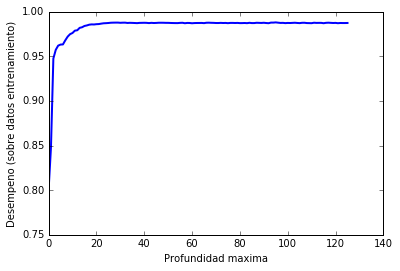
\includegraphics[width=\textwidth]{../imagenes/desempeno-profundiad_arboles}
    \end{subfigure}
    \caption{}
    \label{fig:autovalores}
  \end{figure}


Vemos que el desempeño presenta una fuerte mejora a medida que se aumenta la profundidad máxima 
permitida del árbol hasta profundidades de 15 a 20 niveles. Luego el desempeño 
prácticamente no crece. Para evitarnos posibles problemas de 'overfitting', 
decidimos limitar en 15 la profundidad de los árboles usados con un desempeño 
correspondiente de 0.982.

\subsection{Naive Bayes. NB.}\label{sec:NB}

El m\'etodo de Naive Bayes no result\'o adecuado para este set de datos. El desempeño sobre los datos de entrenamiento fue de tan solo $0.52 \pm 0.01$. 
La hipótesis sobre este mal desempeño es que los atributos elegidos no son lo
suficientemente independientes como para estar dentro de la hipótesis del
método. En la sección \ref{sec:NB_PCA} realizamos un nuevo estudio 
sobre este método, buscando mejorar su eficacia.

\subsection{k-nearest neighbors. KNN}

Para determinar la cantidad de vecinos \'optimo evaluamos el desempeño en cross validation con 10-folds con $k \in \{1,10,20,40,80,160,320,640\} $ vecinos. Los resultados son los siguientes, 

\begin{figure}[H]
  \centering
  \begin{subfigure}[b]{0.4\textwidth}
    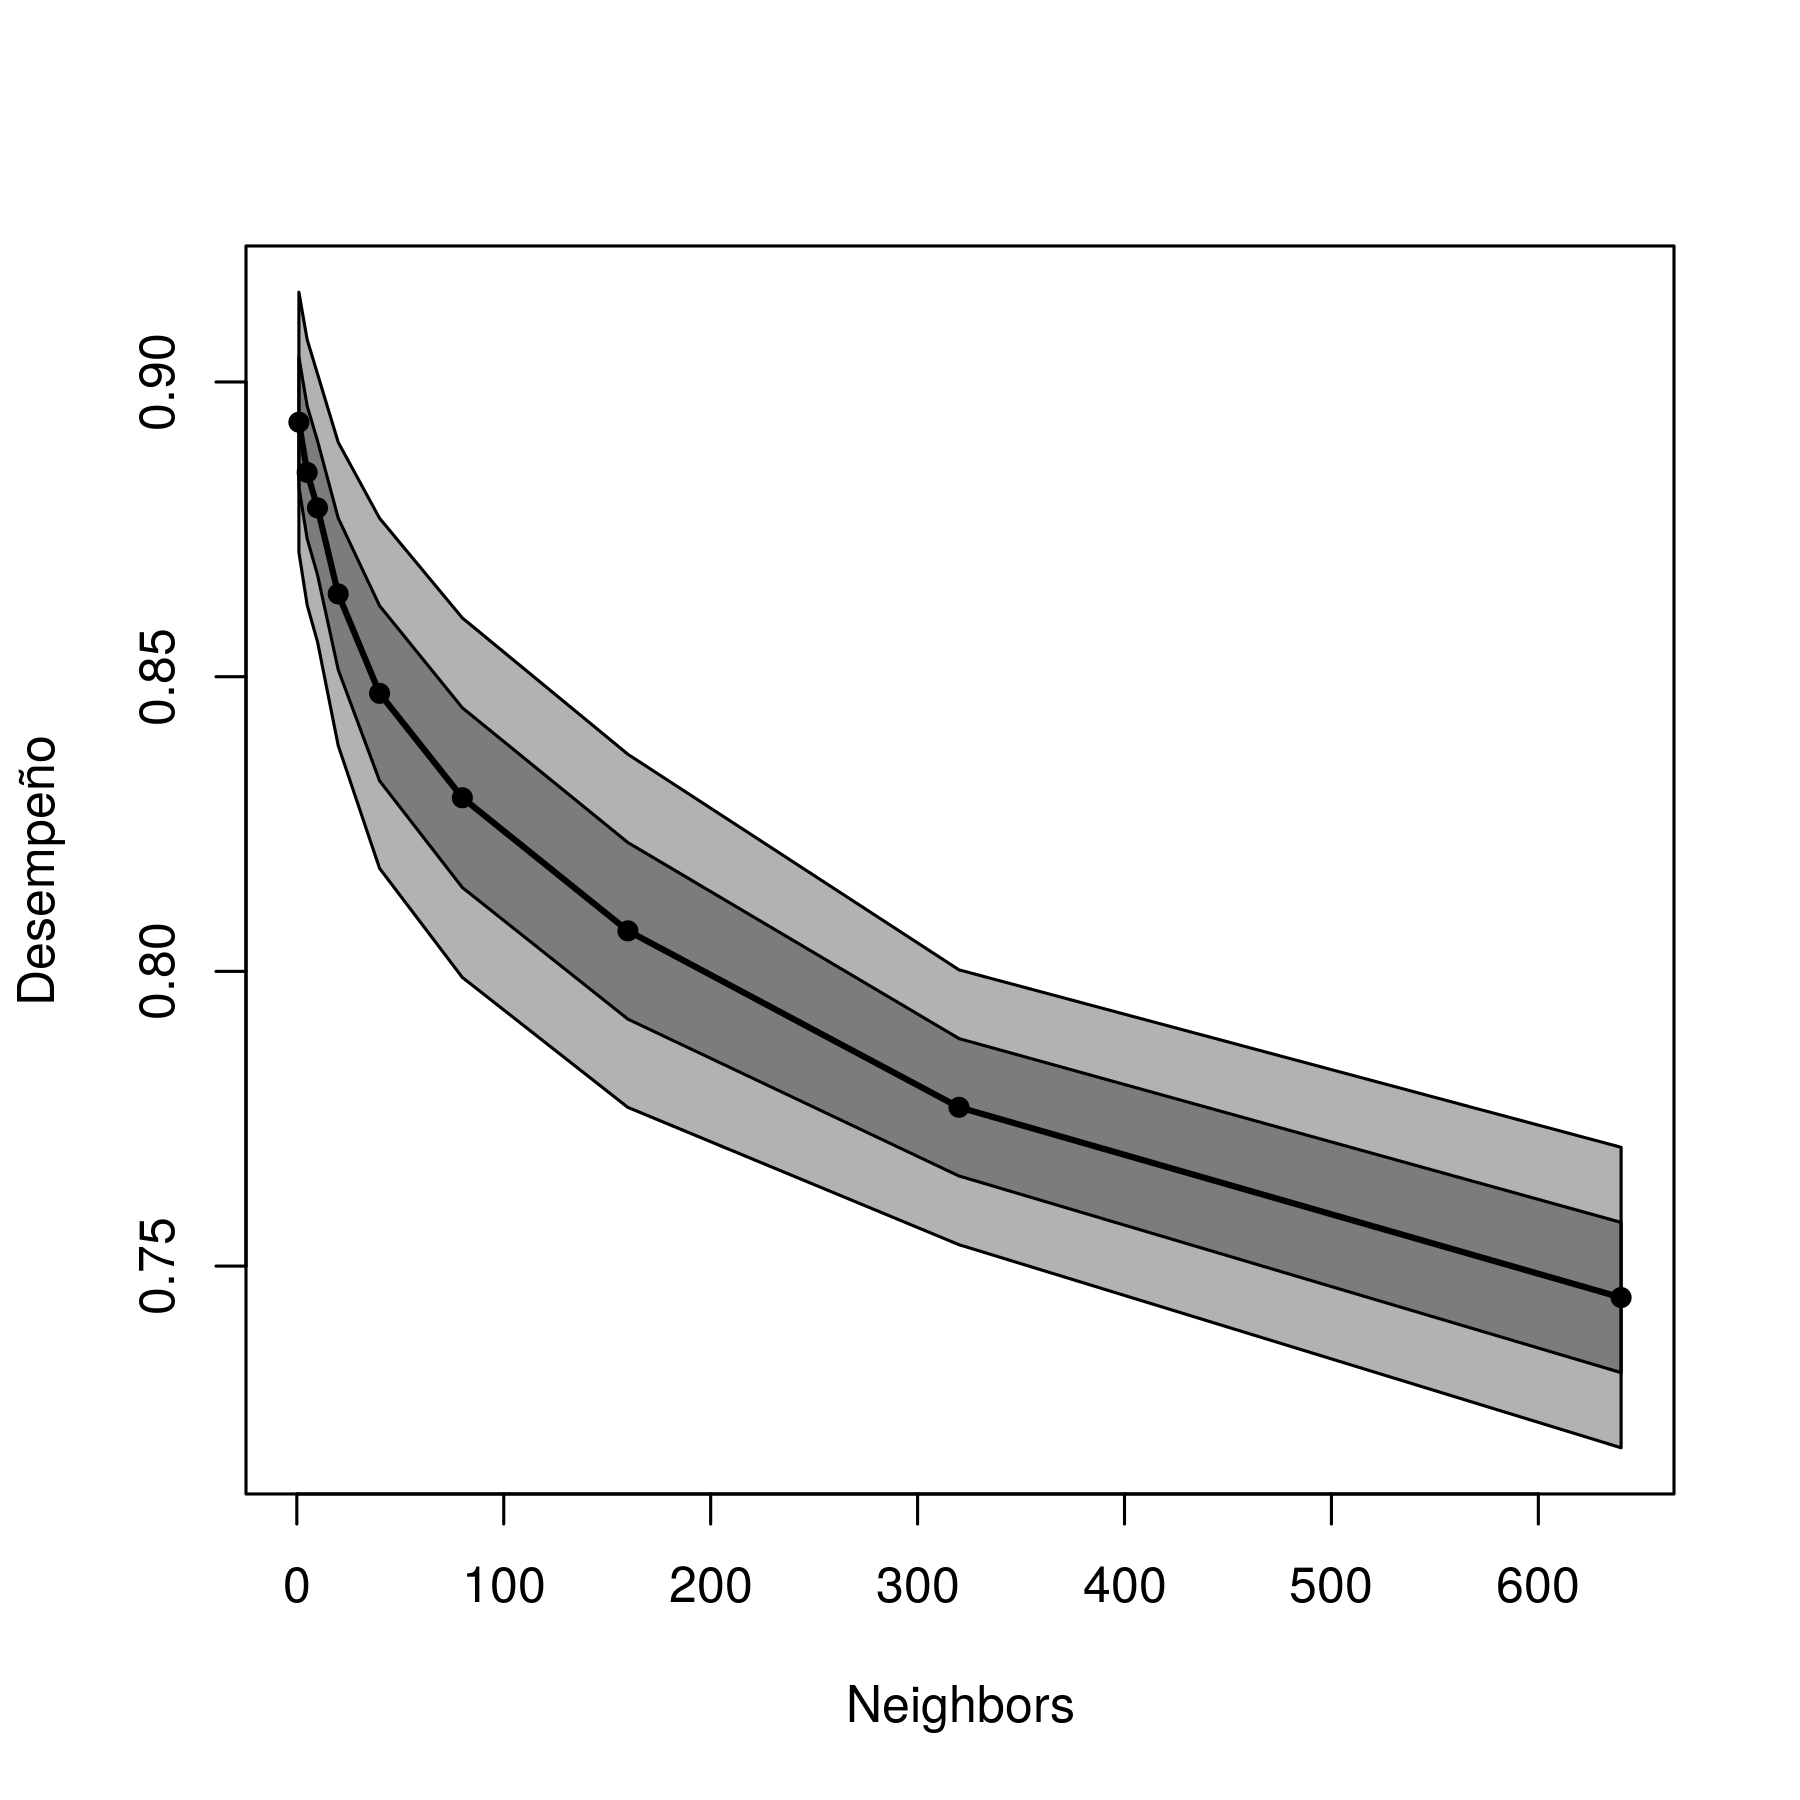
\includegraphics[width=\textwidth]{../imagenes/knn-n_neighbors}
  \end{subfigure}
  \caption{}
  \label{fig:knn-n_neighbors}
\end{figure}

El desempeño m\'aximo fue menor a $0,9$ y result\'o ser bajo en comparaci\'on con otro m\'etodos. Nos sorprendi\'o particularmente que la cantidad de vecinos \'optimo para este problema haya sido con un \'unico vecino. 

\subsection{Random Forest. RF.}

Para determinar la cantidad de \'arboles que genera cada random forest, probamos el rendimiento de la validaci\'on cruzada 10-fold con $t$ \'arboles $t \in \{1,5,10,20,40,80,160,320,640\}$

\begin{figure}[H]
  \centering
  \begin{subfigure}[b]{0.4\textwidth}
    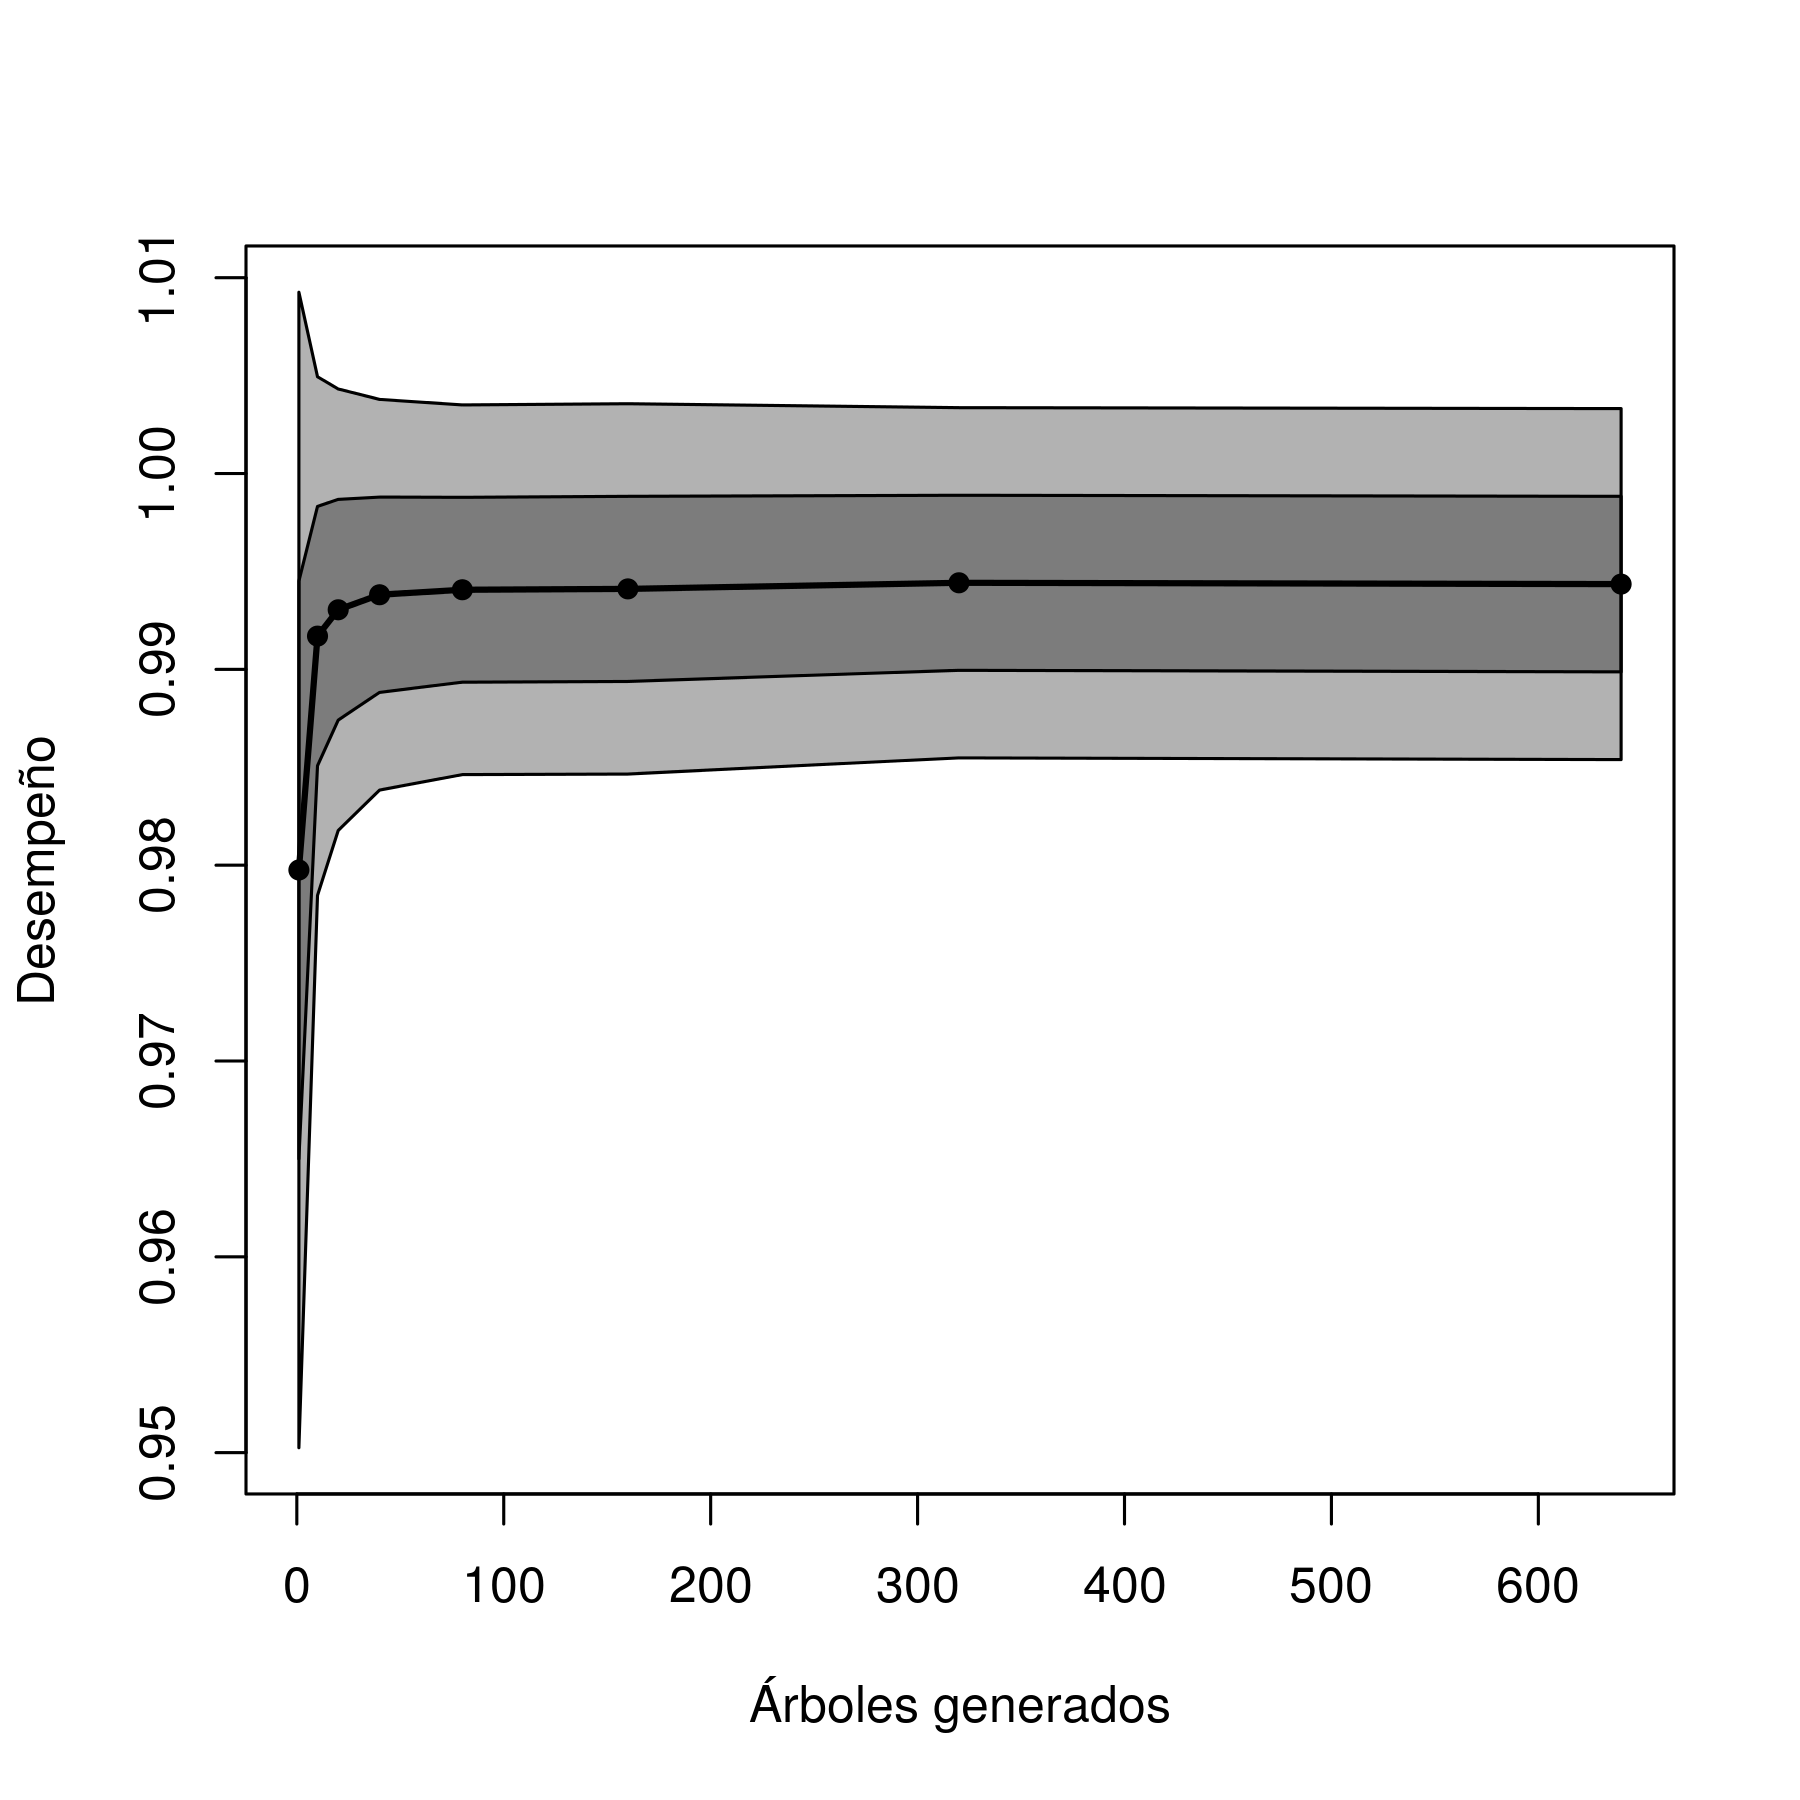
\includegraphics[width=\textwidth]{../imagenes/rf_estimators}
     
  \end{subfigure}
   \caption{}
  \label{fig:rf_estimators}
\end{figure}

40 \'arboles parecen ser suficiente para optimizar el m\'etodo random forest.  

La cantidad m\'axima de atributos $a$ que se utiliza en cada iteraci\'on la dejamos con su valor por defecto $a = \sqrt(|A|)$. En el libro ``An Introduction to Statistical Learning''~\cite{james_hastie_tibshirani} se discute ese tema y se concluye que es una valor bueno en general. 


\subsection{Suport Vector Machine. SVM.}

\par Decidimos realizar el estudio para SVM con un subconjunto del dataset original. Del tutorial de \emph{scikit-learn} (\cite{sklearn}) observamos que la complejidad computacional es cuadrática en el tamaño de la muestra. Este método es muy lento para entrenar y validar con la totalidad de los datos. Por lo tanto utilizamos un dataset acotado a 10000 mails (50\% ham - 50\% spam) con el cual obtuvimos las eficacias de la figura \ref{fig:svm} para distintos kernels y valores del parámetro C, que constituye un valor de tolerancia ante datos mal clasificados.

\begin{figure}[H]
  \centering
  \begin{subfigure}[b]{0.4\textwidth}
    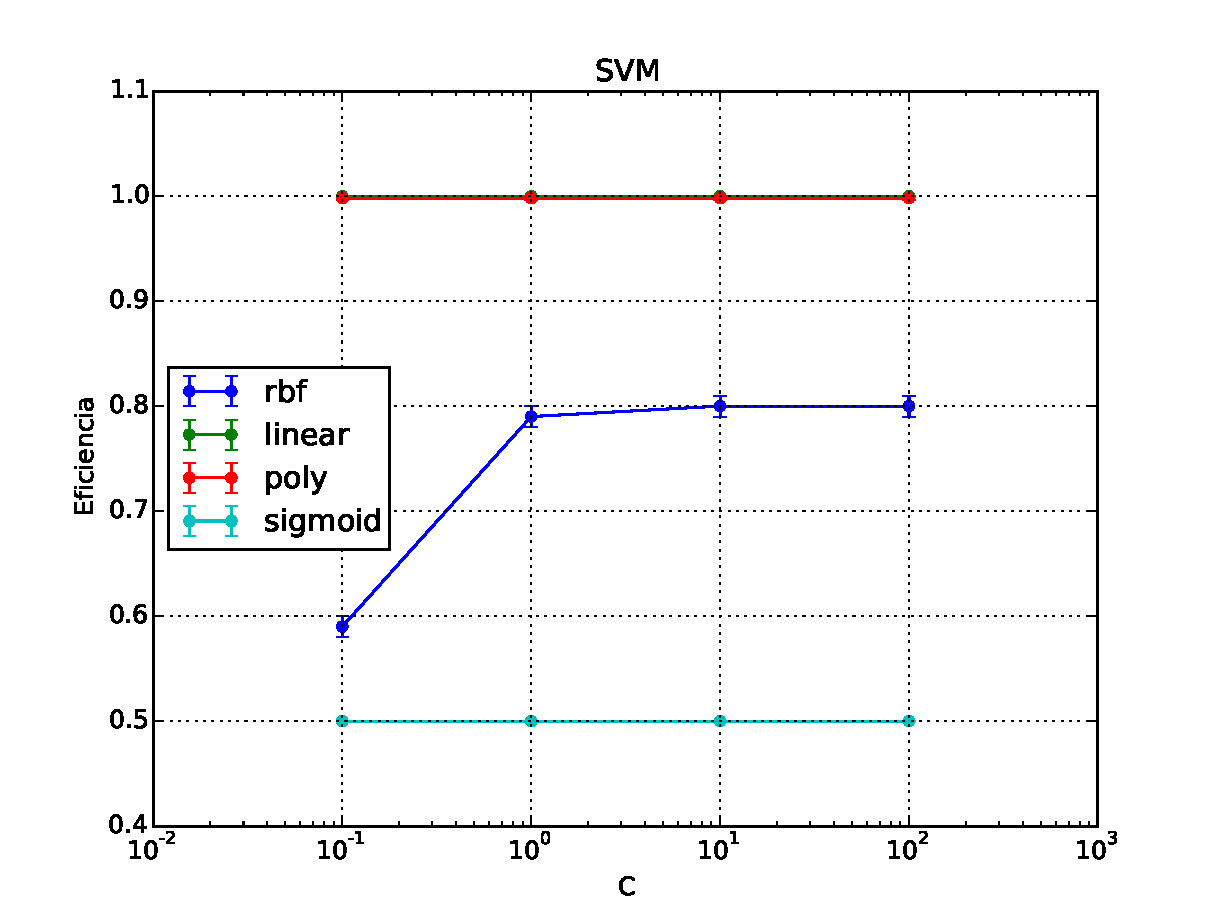
\includegraphics[width=\textwidth]{../imagenes/SVM}    
  \end{subfigure}
    \caption{Eficacia de SVM para distintos kernels y valores de C, para un subconjunto de datos.}
  \label{fig:svm}
\end{figure}

\par Los tiempos de ejecución para cada kernel, promediados para los valores de $C$ empleados son los siguientes:
\begin{table}[H]
\centering
\begin{tabular}{ll}
Kernel & Tiempo (s) \\
Linear & 1850 \\
Poly (degree = 3) & 202 \\
Rbf & 192 \\
Sigmoid & 154 \\
\end{tabular}
\caption{Tiempo de validación de SVM, para distintos kernels.}
\label{table:time_svm}
\end{table}
De la tabla \ref{table:time_svm} y la figura \ref{fig:svm} concluímos que SVM para un los kernels \emph{linear} y \emph{poly} dan una muy buena eficacia, que el tiempo para \emph{linear} es mucho mayor que para \emph{poly}, pero que ambos casos, el tiempo de validación es claramente más alto que los otros métodos estudiados, aún al trabajar con un dataset acotado.


\section{Reducci\'on de dimensionalidad} \label{sec:seleccion}

En esta secci\'on implementamos varios m\'etodos de reducci\'on de dimensionalidad. Optamos por la descomposición en valores singulares (svd) para seleccionar atributos. 

\subsection{Features Ranking}

Evaluamos la ganancia de cada variable individualmente y obtuvimos el siguiente ranking. 

  \begin{figure}[H]
    \centering
    \begin{subfigure}[b]{0.4\textwidth}
      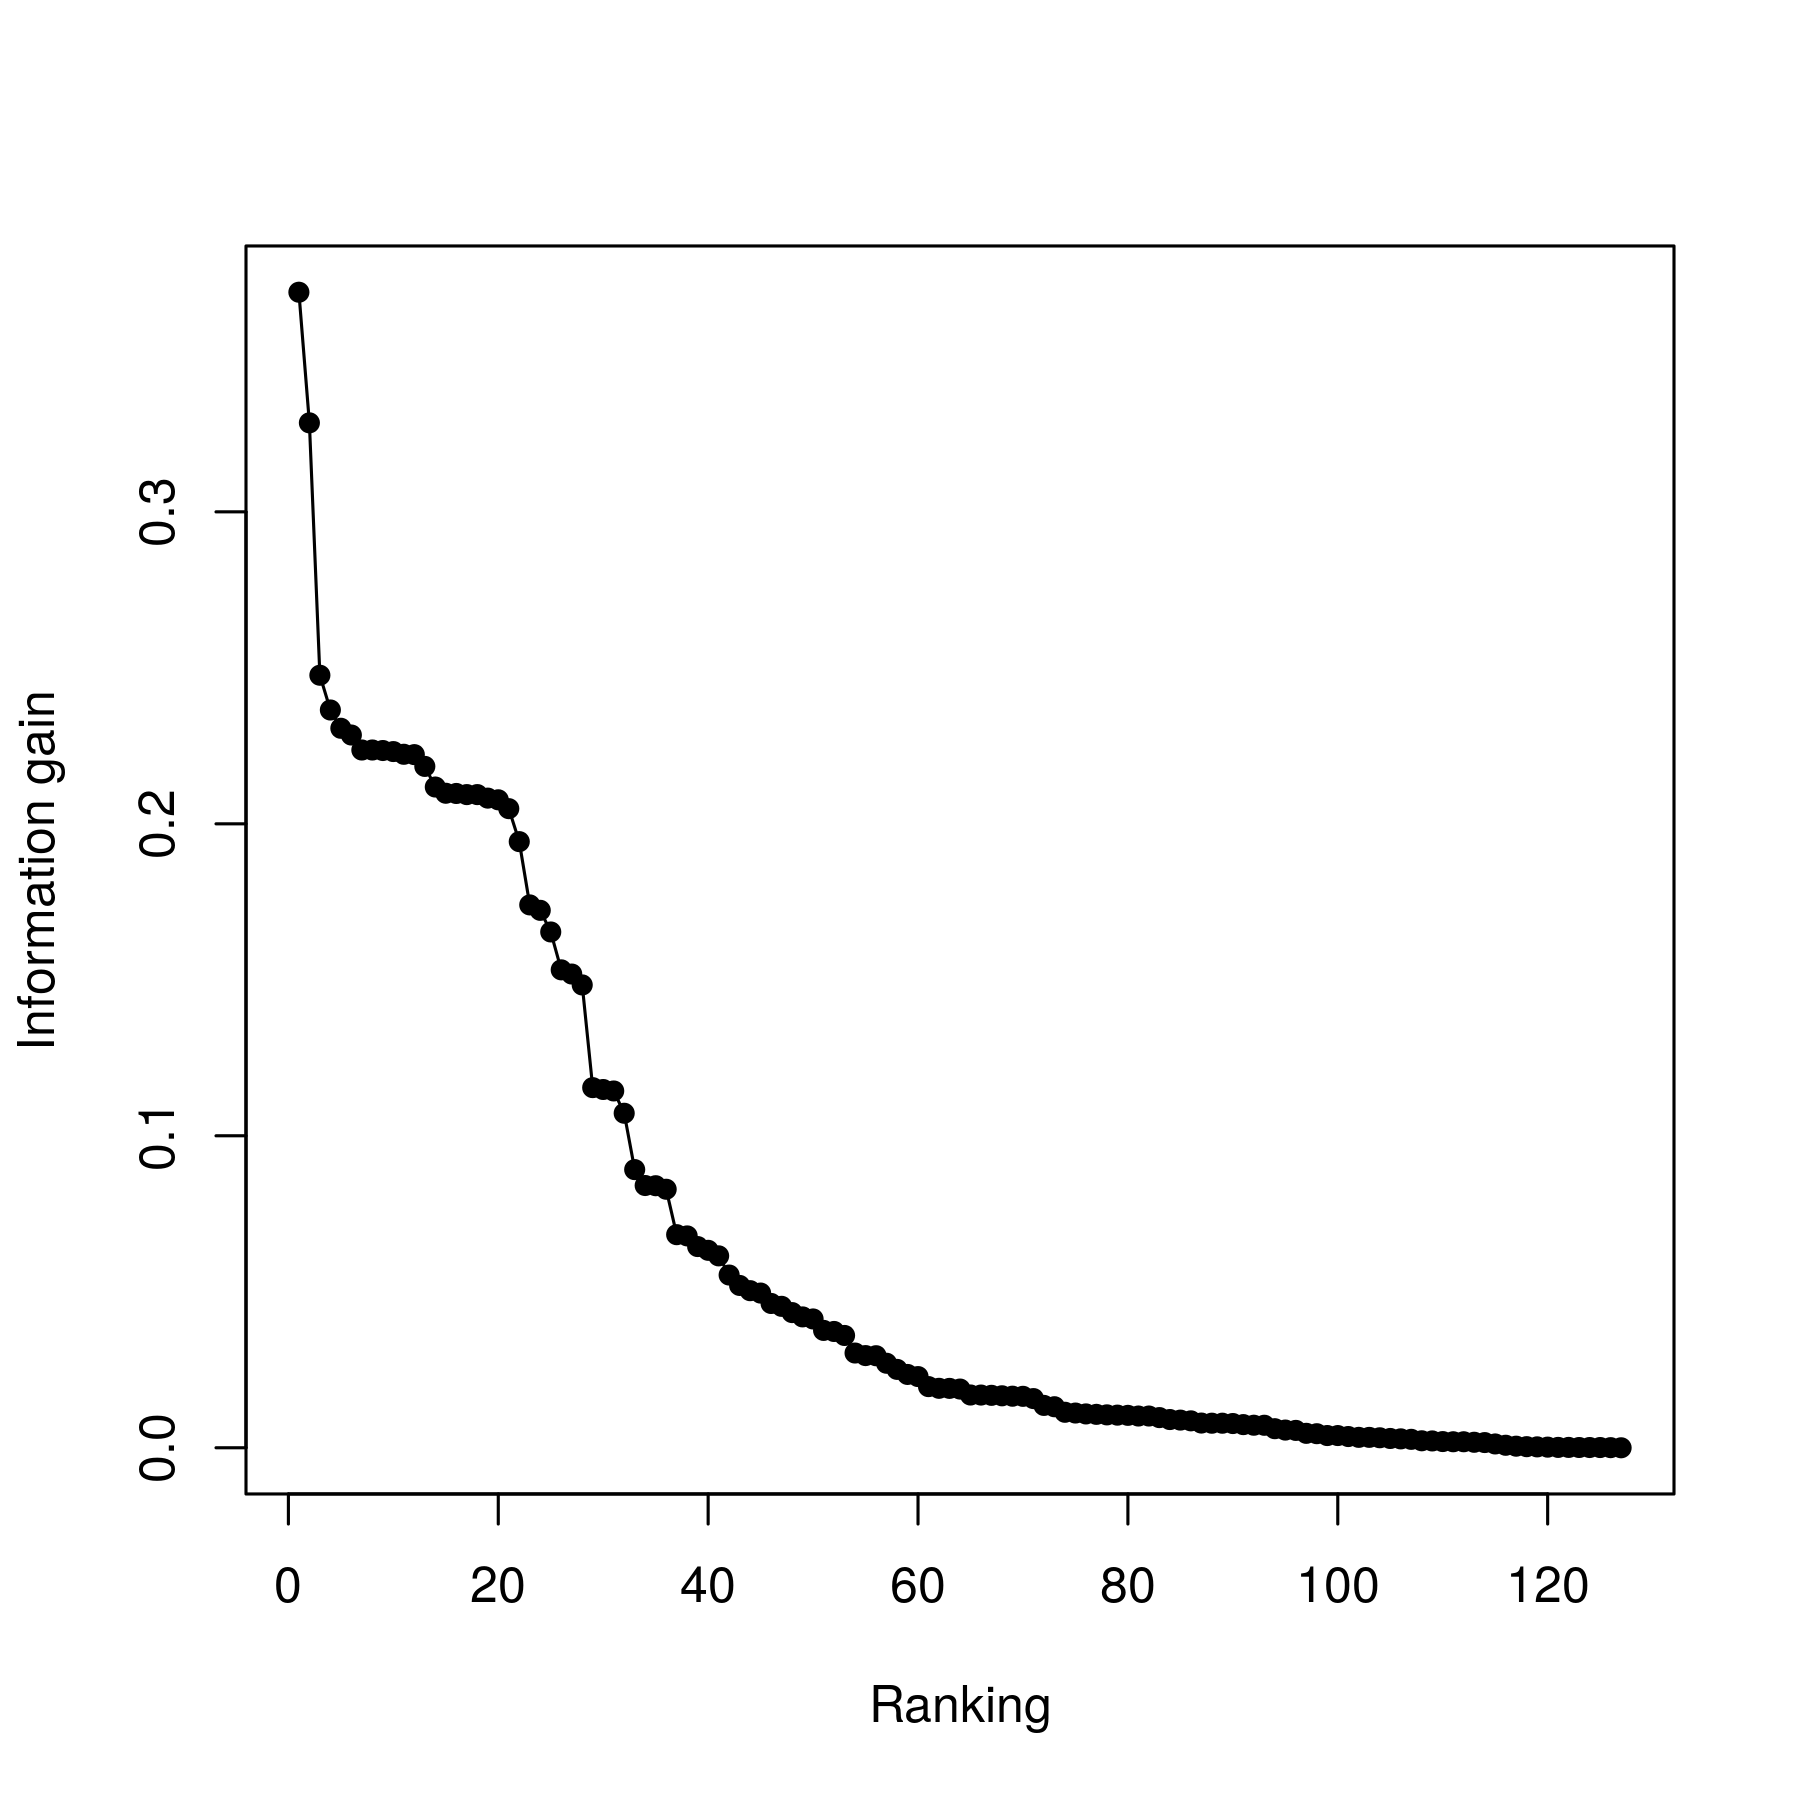
\includegraphics[width=\textwidth]{../imagenes/features_ranking}
     
    \end{subfigure}
      \caption{}
    \label{fig:features_ranking}
  \end{figure}

Este ranking no considera la dependecia entre variables. Dos variables correlacionadas pueden tener individualmente la misma ganancia de informaci\'on, pero al ser tomadas juntas una puede resultar superflua. Para tener en cuenta la interecci\'on implementamos otros m\'etodos. 

\subsection{Hill climbing}

Implementamos completo un algoritmo de hill climibing. Este m\'etodo de selecci\'on de variables busca maximizar la performance resultante de aplicar a un conjunto de datos, $D$, un modelo $L$, evualuado sobre un subconjunto de atributos $S$ variable. La vecindad de un subconjunto $S$ son todos los subconjuntos que se pueden contruir sacando de $S$ un \'unico elemento, o agregando a $S$ un \'unico elemento. Corrimos 50 procesos de hill climbing evaluando la perfomance en cada punto ejecutando un \'arbol de decisi\'on con cross validation 5-fold. Encontramos 50 \'optimos locales, sin repetici\'on. Las performance de los \'optimos locales estuvieron entre 0.88 y 0.96. Este proceso no fue suficiente para decidir por un \'unico subconjunto de atributos para la selecci\'on de atributos. 

La performance que se obtiene de la validaci\'on cruzada depende de la partici\'on utilizada. Esa variabilidad puede hacer que ciertos subconjuntos $S$ sean a veces consideramos \'otpimos locales y otras veces no. Una forma de solucionar esto ser\'ia realizar validaci\'on cruzada \emph{leave one out}, pero este m\'etodo es muy costoso. Otra opci\'on es fijar 5-folds iguales para todos las pruebas de validaci\'on cruzada y considerar \'unicamentre la performance obtenida sobrea esa partici\'on particular.  

Sin embargo, las diferencias entre los \'otpimos locales obtenidos no fueron significativas para determinar con certeza un \'unico subconjunto de variables. Para eso implementamos otro m\'etodo. 

\subsection{Principal Component Analysis. PCA}

\par De los atributos seleccionados, realizamos un reducción de la dimensionalidad
mediante la técnica de PCA. Dada la matriz de \emph{mails} x \emph{atributos},
calculamos la matriz de covarianza de los atributos, y realizamos una descomposición en valores singulares (SVD) mediante la funci\'on \emph{scipy.linalg.svd} \cite{scipy}. La matriz de covarianza es una matriz simétrica, por lo tanto sus valores singulares coinciden con sus autovalores, que además son reales y no negativos. En la figura \ref{fig:autovalores}, observamos el valor de los mismos, ordenados de mayor a menor. 
  \begin{figure}[H]
    \centering
    \begin{subfigure}[b]{0.4\textwidth}
      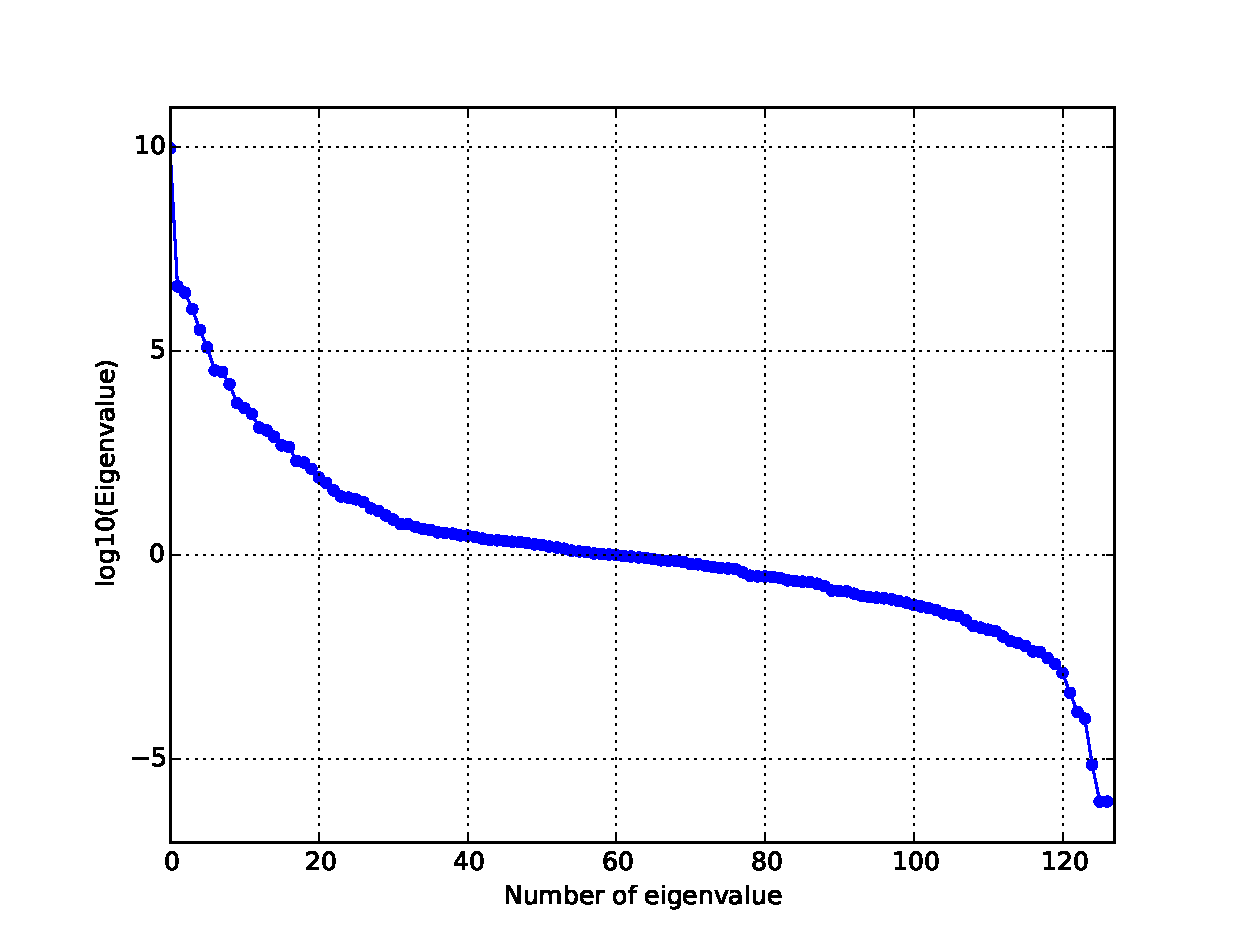
\includegraphics[width=\textwidth]{../imagenes/Autovalores}
    \end{subfigure}
    \caption{Valor de los autovalores surgidos de la descomposición SVD, ordenados de derecha a izquierda.}
    \label{fig:autovalores}
  \end{figure}

\par Los autovectores obtenidos de la factorización son una combinación lineal de los atributos elegidos originalmente. Dichos autovectores pueden ser tomados como nuevos atributos, los cuales, a partir de sus autovalores asociados, sabemos en cuáles hay una mayor variabilidad de los datos. 
\par Para dar una interpretación a los nuevos atributos, observamos la representación de los autovectores en el espacio de atributos originales. Como criterio, estudiamos qué componentes tienen un valor absoluto mayor a $0.1$ en el espacio de atributos originales. En la tabla \ref{table:autovectores} mostramos el resultado para las 5 direcciones principales. De la tabla vemos que las dos direcciones principales prácticamente coindicen con dos de los atributos elegidos originalmente, asociados al formato del mail en cuestión. Los autovectores siguientes se constituyen de un grupo de términos, de los cuales el 4º y 5º autovector muestran una correlación en la terminología (o procedencia) de los miembros del grupo más visible que en el 3º autovector. 
\begin{table}[H]
\centering
\begin{tabular}{ll}
Autovector & Componentes principales \\
1 & Largo del documento. \\
2 & Cantidad de espacios en blanco. \\
3 & Términos: germ, hi, how, think, valuable, enron, republic, content-class, thread-index. \\
4 & Términos: x-origin, x-filename, x-cc, binary \\
5 & Términos: receive, email, upgrade, fast, spam \\
\end{tabular}
\caption{Principales componentes de los autovectores surgidos de PCA}
\label{table:autovectores}
\end{table}

\subsubsection{Naive Bayes + PCA}\label{sec:NB_PCA}

\par El método de Naive Bayes no resultó satisfactorio para el dataset original, como reportamos en la sección \ref{sec:NB}. La principal hipótesis de tan mal desempeño, fue el hecho de que Naive Bayes suponga que los atributos son independientes entre sí. Por lo tanto, esper\'abamos que con los nuevos atributos obtenidos mediante la técnica PCA, el método funcione mejor, debido a que dichos atributos se construyen buscando ortogonalidad entre los mismos, resultando en atributos más descorrelacionados que los atributos originales entre sí. En la tabla \ref{table:NB} reportamos los valores de eficacia, donde prácticamente no se ven diferencias en tomar un subconjunto de atributos surgidos de PCA y el desempeño original. \footnote{Cuando estudiamos el caso de Naive-Bayes con el dataset original, encontramos grandes diferencias en los resultados obtenidos, según en qué ordenador corríamos el script. El problema estaba en una diferencia de versiones de la librería \emph{scikit-learn}. Los resultados reportados se corresponden con la versión 0.17.1.}

\begin{table}[H]
\centering
\caption{}
\label{table:NB}
\begin{tabular}{lll}
Cantidad de atributos & Eficacia & error \\
5 & 0.51 & 0.01 \\
10 & 0.52 & 0.02 \\
20 & 0.52 & 0.01 \\
120 & 0.51 & 0.01 \\
original & 0.52 & 0.01 \\
\end{tabular}
\end{table}

\subsubsection{knn + PCA}

Al evaluar el clasificador $knn$ sobre las variable transformadas, la cantidad de vecinos \'optimo fue nuevamente $k=1$. En la siguiente figura se muestra el resultado con $k=1$ y $k=10$ al aumentando la cantidad de atributos que se utilizan para clasificar.  

\begin{figure}[H]
  \centering
  \begin{subfigure}[b]{0.4\textwidth}
    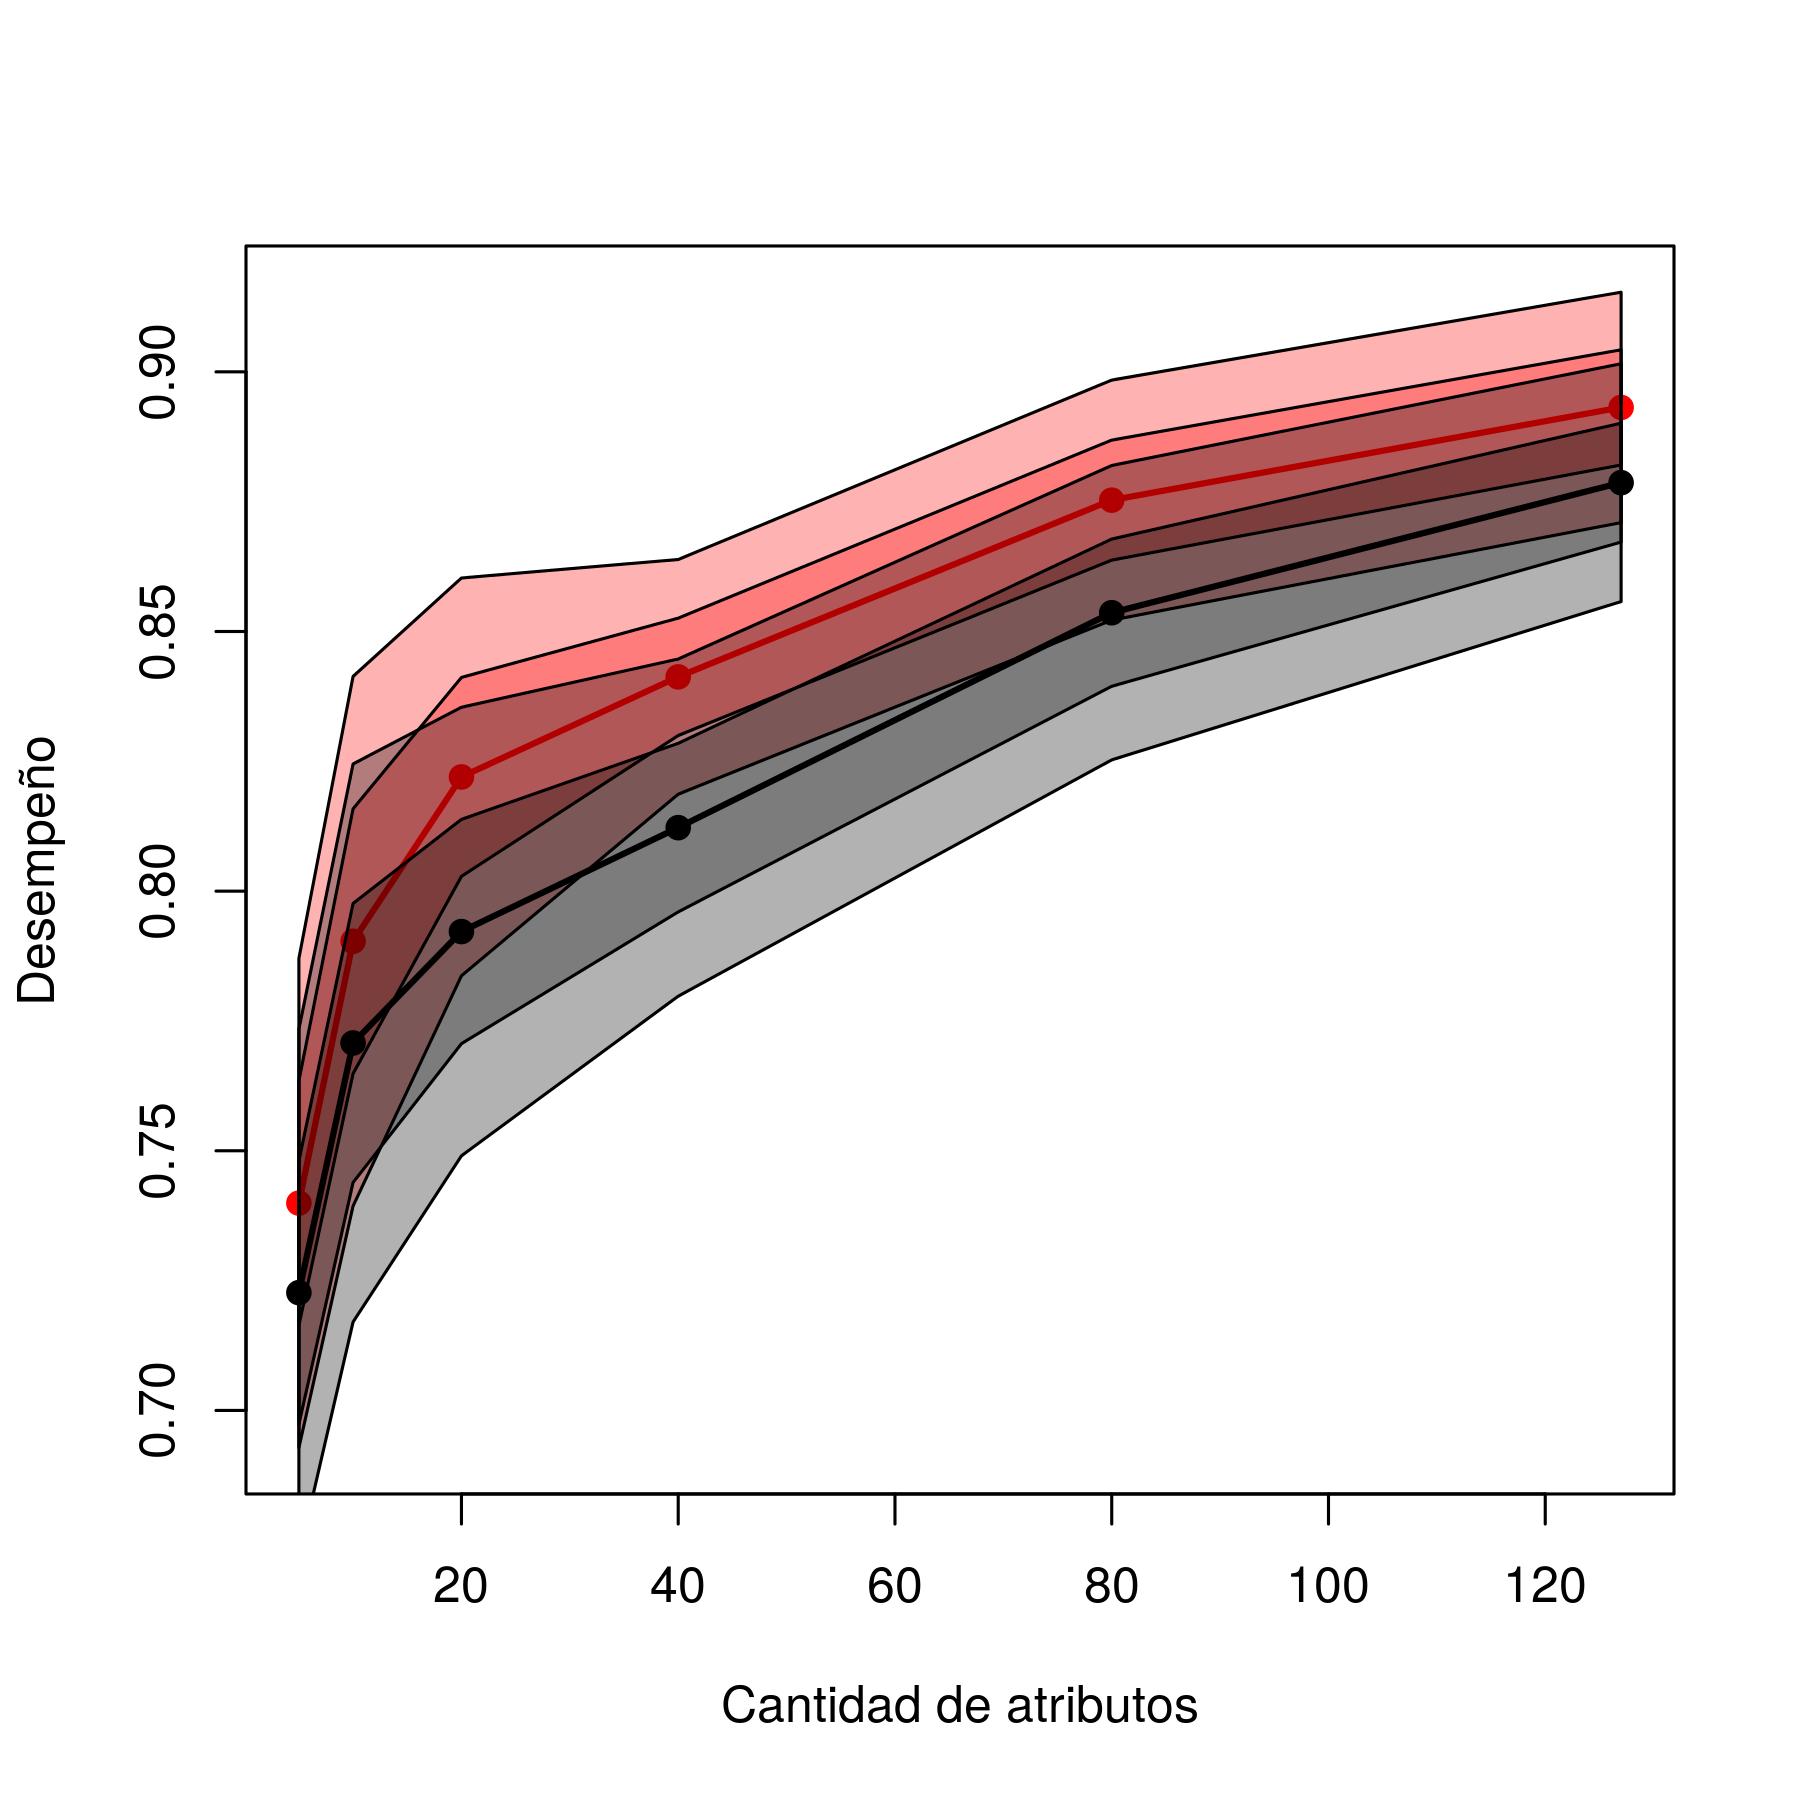
\includegraphics[width=\textwidth]{../imagenes/knn}
  \end{subfigure}
  \caption{Rojo: $k=1$. Negro: $k=10$ }
  \label{fig:knn-n_neighbors}
\end{figure}

Tampoco se observa una mejora con respecto a los atributos no transformados

\subsubsection{árboles + PCA}

Fijamos los parámetros a partir del análisis ya realizado,
Máxima profundidad: 15
Criterio: Gini
Splitter: Best

La figura siguiente muestra el desempeño en función del número de componentes.

Intertar figura "desempeño_vs_componentes_arboles" porfa.

Como esperabamos, el desempeño crece abruptamente al comienzo para luego hacerlo en forma moderada hasta la componente 43 cuando se alcanza prácticamente el valor máximo. Parece entonces ser esa una cantidad adecuada de componentes a considerar.

\subsubsection{random forest + PCA}

Probamos random forest con 40 \'arboles con $v$ variables en el nuevo sistema de coordenadas, $v \in \{5,10,20,40,127\}$

\begin{figure}[H]
  \centering
  \begin{subfigure}[b]{0.4\textwidth}
    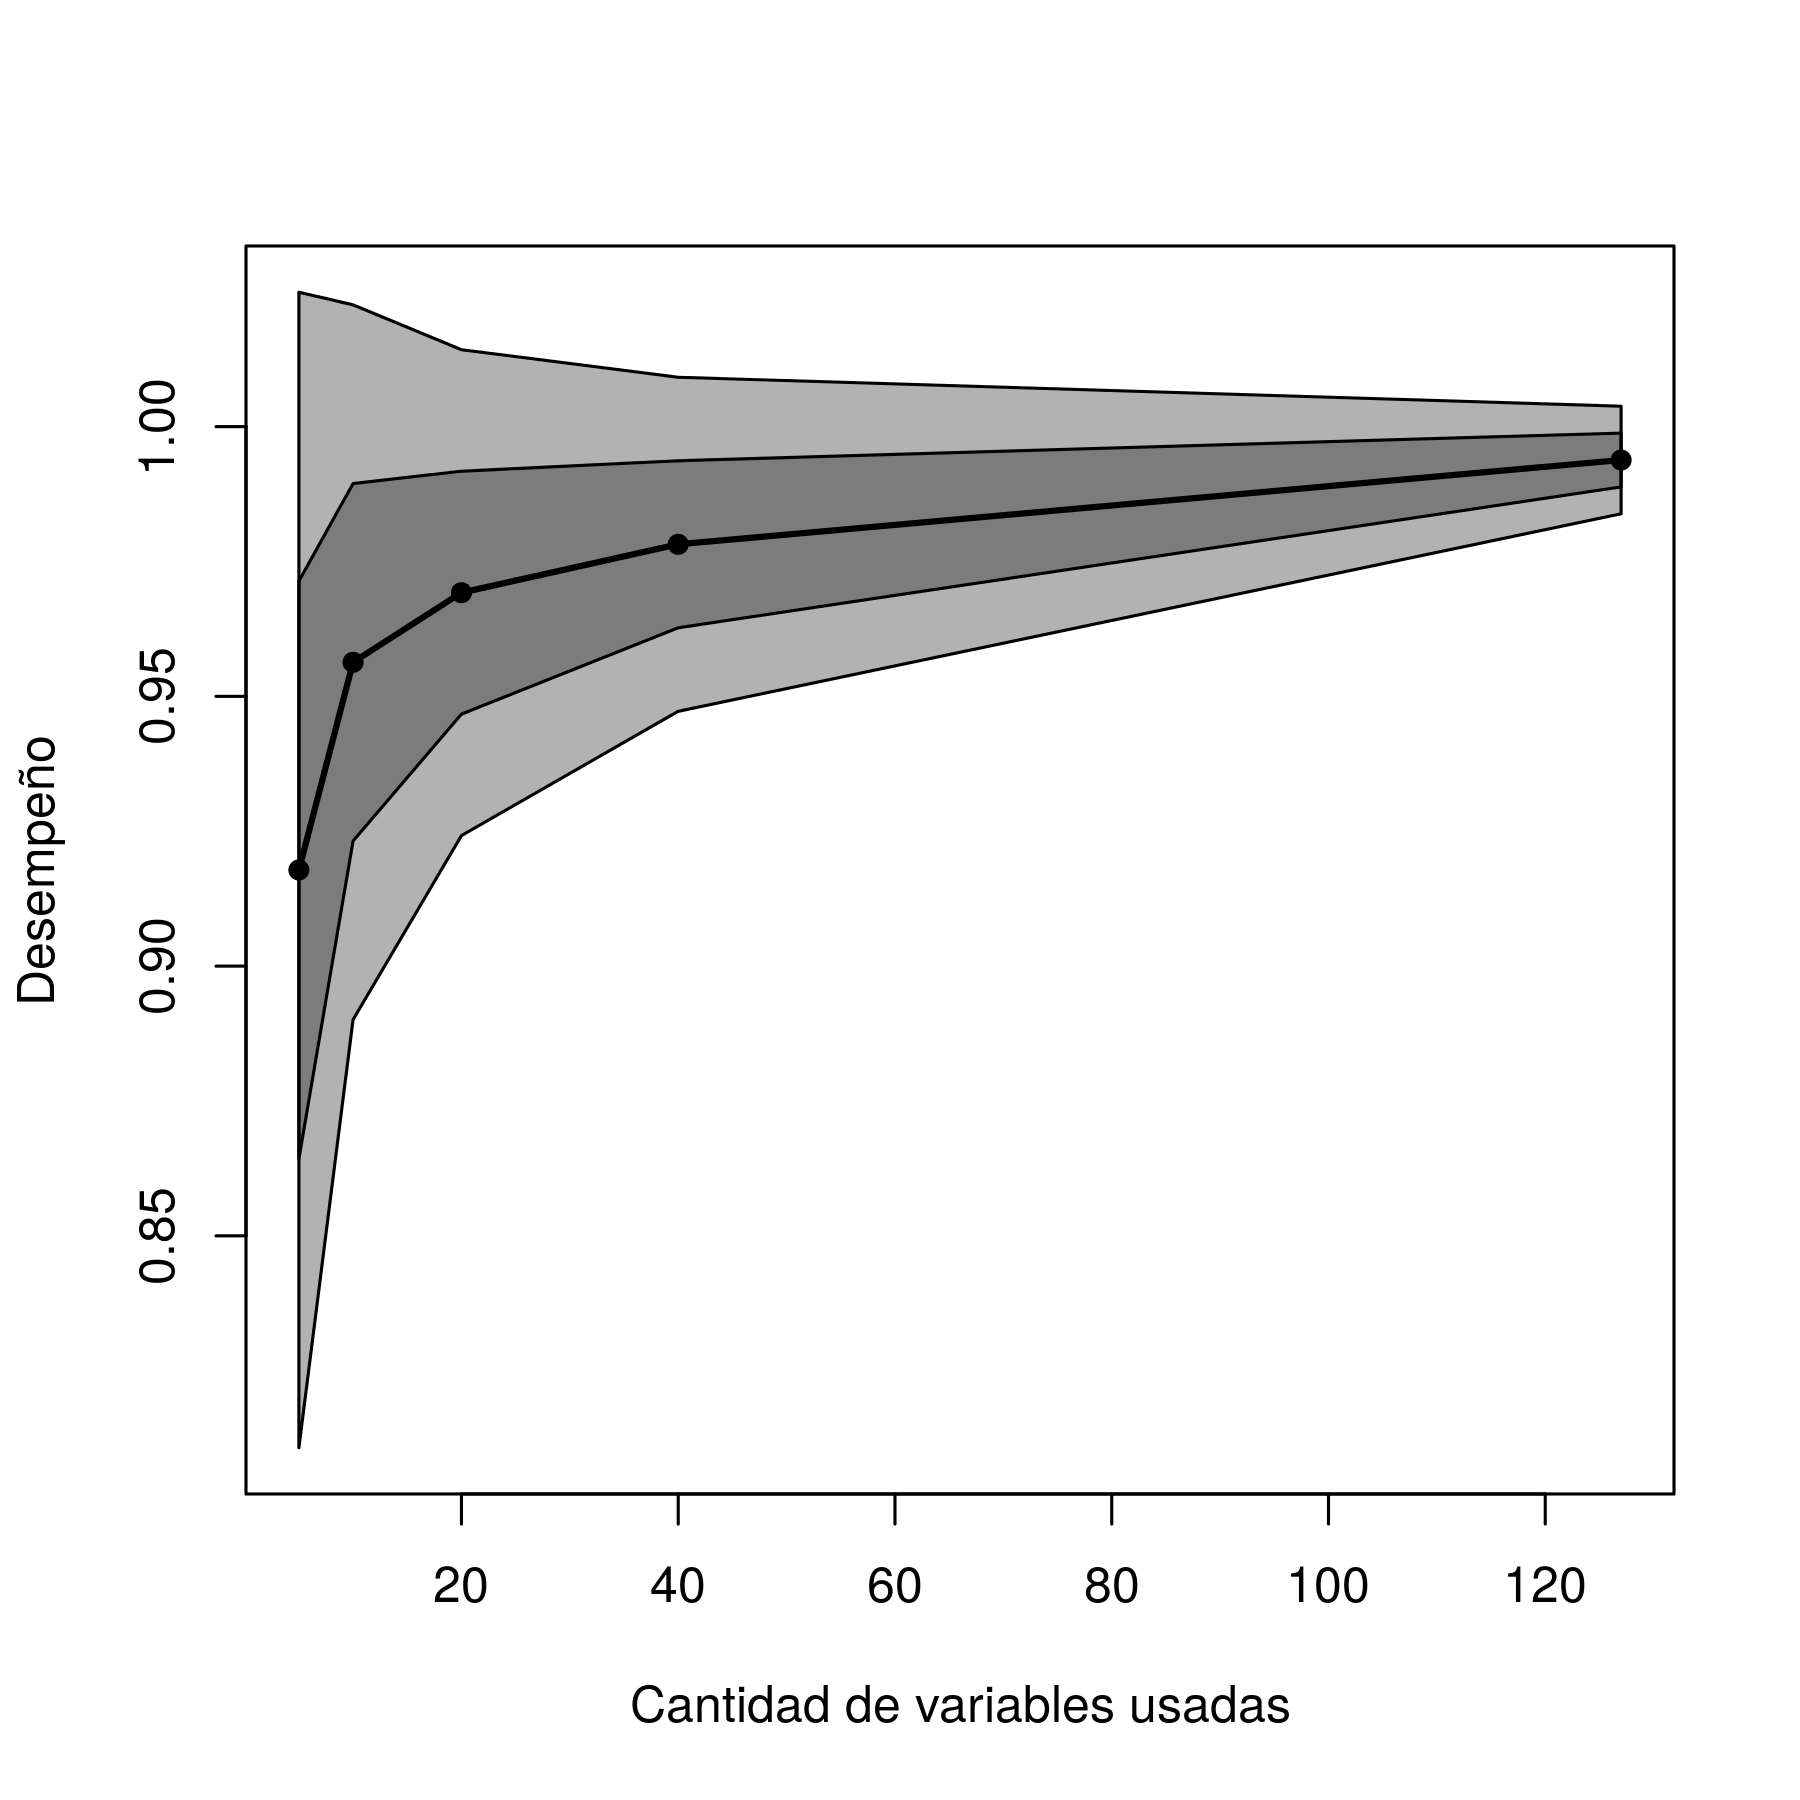
\includegraphics[width=\textwidth]{../imagenes/rf}
     
  \end{subfigure}
  \caption{}
  \label{fig:rf}
\end{figure}

No se observa mejora con respecto a los atributos no transformados. 

\subsubsection{SVM + PCA}

\par Estudiamos el caso de SVM con kernel polinomial y variables reducidas, sin embargo el tiempo de ejecución se incrementó significativamente respecto al caso de tomar todas los atributos originales, por lo que descartamos que sea una mejora para este modelo.

\section{Resultados y conclusiones}

\par Luego de analizar diferentes modelos, concluimos que los métodos que mostraron una mejor performance para el conjunto de atributos son SVM y Random Forest, teniendo el último un tiempo de validación y entrenamiento considerablemente menor que el primero.
\par La generación de nuevos atributos mediante la reducción de dimensionalidad con técnicas tales como PCA, no supuso una mejora significante en el balance entre tiempo de ejecución y eficacia de los modelos. 
\par Por otro lado, vale destacar que los resultados reportados corresponden de realizar un promedio de los rendimientos obtenidos al hacer \emph{cross-fold validation}, por lo que somos concientes que podemos estar realizando un \emph{over-fitting} sobre los datos analizados, y la perfomance de los modelos ante una base de datos nueva puede diferir de la predicha en este trabajo. 

\section{Discusi\'on}

Algunos hechos que fueron surgiendo a medida que se desarrollaba el trabajo pr\'actico, que al principio nos parec\'ian eventos aislados, pensamos que pueden ser considerados en realidad como un indicio de un problema originado en la extracci\'on de atributos. Los hechos aparentemente aislados ser\'ian

\begin{itemize}
 \item La baja performance de \emph{naive bayes}. 
 \item El cantidad de vecinos \'optimo para determinar la clase mediante \emph{KNN} igual a 1. 
 \item La variedad de \'optimos locales al realizar \emph{hill climbing}. 
\end{itemize}

Hoy suponemos que la baja performance de naive bayes se debe a una fuerte dependencia entre los atributos. A su vez pensamos que la cantidad de vecinos \'optimo para knn sea un \'unico vecino podr\'ia estar indicando que los datos no est\'an bien separados en el espacio, es decir, que los atributos no distinguen con suficentemente claridad una clase de otra. Finalmente sospechamos que la variedad de \'optimos locales se debe a la alta correlaci\'on entre los datos. 
Algunas cosas que deber\'iamos implementar para mejorar para la extracci\'on de atributos 

\begin{itemize}
 \item Sacar el encabezado del mail para la selecci\'on de palabras. 
 \item Sacar el html para la selecci\'on de palabras. 
 \item Estandarizar los string de tipo archivo adjunto (m\'as de tres aaa) como una \'unica variable 
\end{itemize}






\scriptsize
\bibliographystyle{splncs03}
\bibliography{aa}



\end{document}

